\chapter{IMPLEMENTATION}
Data dependency generation is implemented as an \code{angr} analysis and is registered under the name ‘DataDep’. This allows the \code{angr} library user to access and utilize DDG functionalities through \code{project.analyses.DataDep()}. To maintain interoperability between DataDep and other \code{angr} analyses, the analysis outputs an instance of a NetworkX Digraph representing the generated DDG \citep{networkx}. The generated graph can then be further operated upon by the user or visualized using standard NetworkX visualization techniques \citep{networkxdraw}

In order to generate a DDG, the analysis must be provided a symbolic execution state which acts as a source of data moves performed by the program. This state is referred to as an “end-state”, as it provides a history containing all the reads and writes taken by the program up until a given endpoint. In \code{angr}, these simulated read and write actions are encapsulated in $SimActionDatas$. As far as \code{angr} is concerned, an action can be one of the types seen in Table \ref{table:types}.

\begin{table}
    \begin{center}
        \caption[Supported Action Types]{Supported Action Types.}
        \label{table:types}
        \begin{tabular}{ |c|c| }
        \hline
        \textbf{Type of Action} & \textbf{AMD64 Example} \\
        \hline
        A read from a `variable' & \code{mov rdx, rdi} (in terms of \code{rdi}) \\
        \hline
        A write to a `variable' & \code{mov rdx, rdi} (in terms of \code{rdx}) \\
        \hline
        A read from a memory address & \code{mov r9, [rax]} \\
        \hline
        A write to a memory address & \code{mov dword ptr [rax], 0xdeadbeef}) \\
        \hline
        \end{tabular}
    \end{center}
\end{table}

As naively ingesting an end state that captures all the reads and writes performed by a large program would result in a tremendous and unwieldy number of nodes for the user to parse through, the analysis supports a finer-grained approach by tailoring the graph to a portion of code of interest. This is accomplished by providing a symbolic execution state that begins its execution at the earliest point in time of concern and ends its execution on the instruction one beyond the latest point in time of concern. This “end-state” serves as the execution trace that must be provided along with the binary in question. The user may also optionally specify the block instructions or range of instruction addresses to include in the graph.

\section{Dependency Nodes}
The analysis operates on four distinct classes of nodes: memory, register, temporary, and constant. The first three types of nodes are used to represent a MEM, REG, and TMP \code{SimActionData}, respectively. The final nodal type, constant, is used to represent any untracked, literal value written or read from a \code{SimActionData}. As constants cannot, by definition, be dependent upon any other node. In other words, one cannot write to the decimal value 470. Thus, constants will always appear as the highest-level ancestors in a DDG. Each of these node types is represented by a corresponding class of nodes used by the analysis. The inheritance relationships between these classes, as seen in Figure \ref{fig:dep} is explained in greater detail below.

\begin{figure}
    \centering
    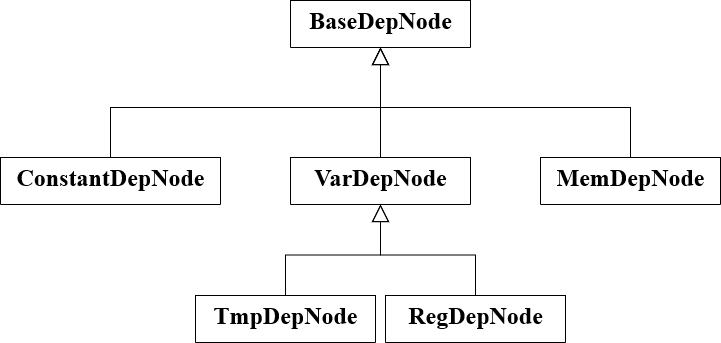
\includegraphics[width=0.8\maxwidth{\textwidth}]{dep.png}
    \caption[UML Diagram of Dependency Node Class Inheritance]{UML diagram of dependency node class inheritance. All nodes in a generated data dependency graph are represented by the leaf classes in this figure, with all other classes being abstract.}
    \label{fig:dep}
\end{figure}


\subsection{Base Dependency Nodes}
The base dependency node class is abstract and serves as a template for what attributes its descendant classes must have. This class defines that, at a minimum, a node possesses a class type, instruction address, statement index, and action identifier. While the instruction address and statement index is straightforward, being the instruction of the address in which the dependency node resides and the index of the statement in that address respectively, the action warrants explanation. The action identifier is sourced directly from the node’s corresponding \code{SimActionData} and is a unique counter marking the occurrence of the given action in the entire program’s execution. 

\subsection{Constant Dependency Nodes}
The constant dependency nodes class is concrete and represented in a generated DDG. It is solely identified by its value.

\subsection{Memory Dependency Nodes}
The memory dependence nodes class is also concrete and represented in a generated DDG. In addition to the attributes that identify a base dependency node, a memory dependency node is further identified by its memory address. 

\subsection{Variable Dependency Nodes}
The variable dependency nodes class is abstract, serving as a common ancestor to temporary and register dependency nodes. While temporary and register nodes are different types of \code{SimActions}, both are identified by a register number and can be parsed without needing to be differentiated. 

\subsection{Temporary Dependency Nodes}
\label{section:tmp}
The temprorary dependency nodes class is concrete and represented in a generated DDG. While it adds no additional functionality to its base class, it is included in order to differentiate between register and temporary nodes for ease of filtering the graph for display. As the number of temporary nodes will be high for a given program, it is often beneficial to hide them in a generated DDG. 

\subsection{Register Dependency Nodes}
The register dependency nodes class is concrete and represented in a generated DDG. It exists to differentiate between register and temporary nodes for the reasons proposed in Section \ref{section:tmp}

\section{Generating and Tracking Nodes}
Based on the type and action of the \code{SimActionData} currently being parsed, different fields are pulled out of the action to create the respective dependency node. Upon creating a node for an action, the action is popped from the parsing queue and the node is added to the graph. The node is originally unconnected, as it has yet to be linked to the DDG.  

\section{Linking Nodes}
\begin{figure}
    \centering
    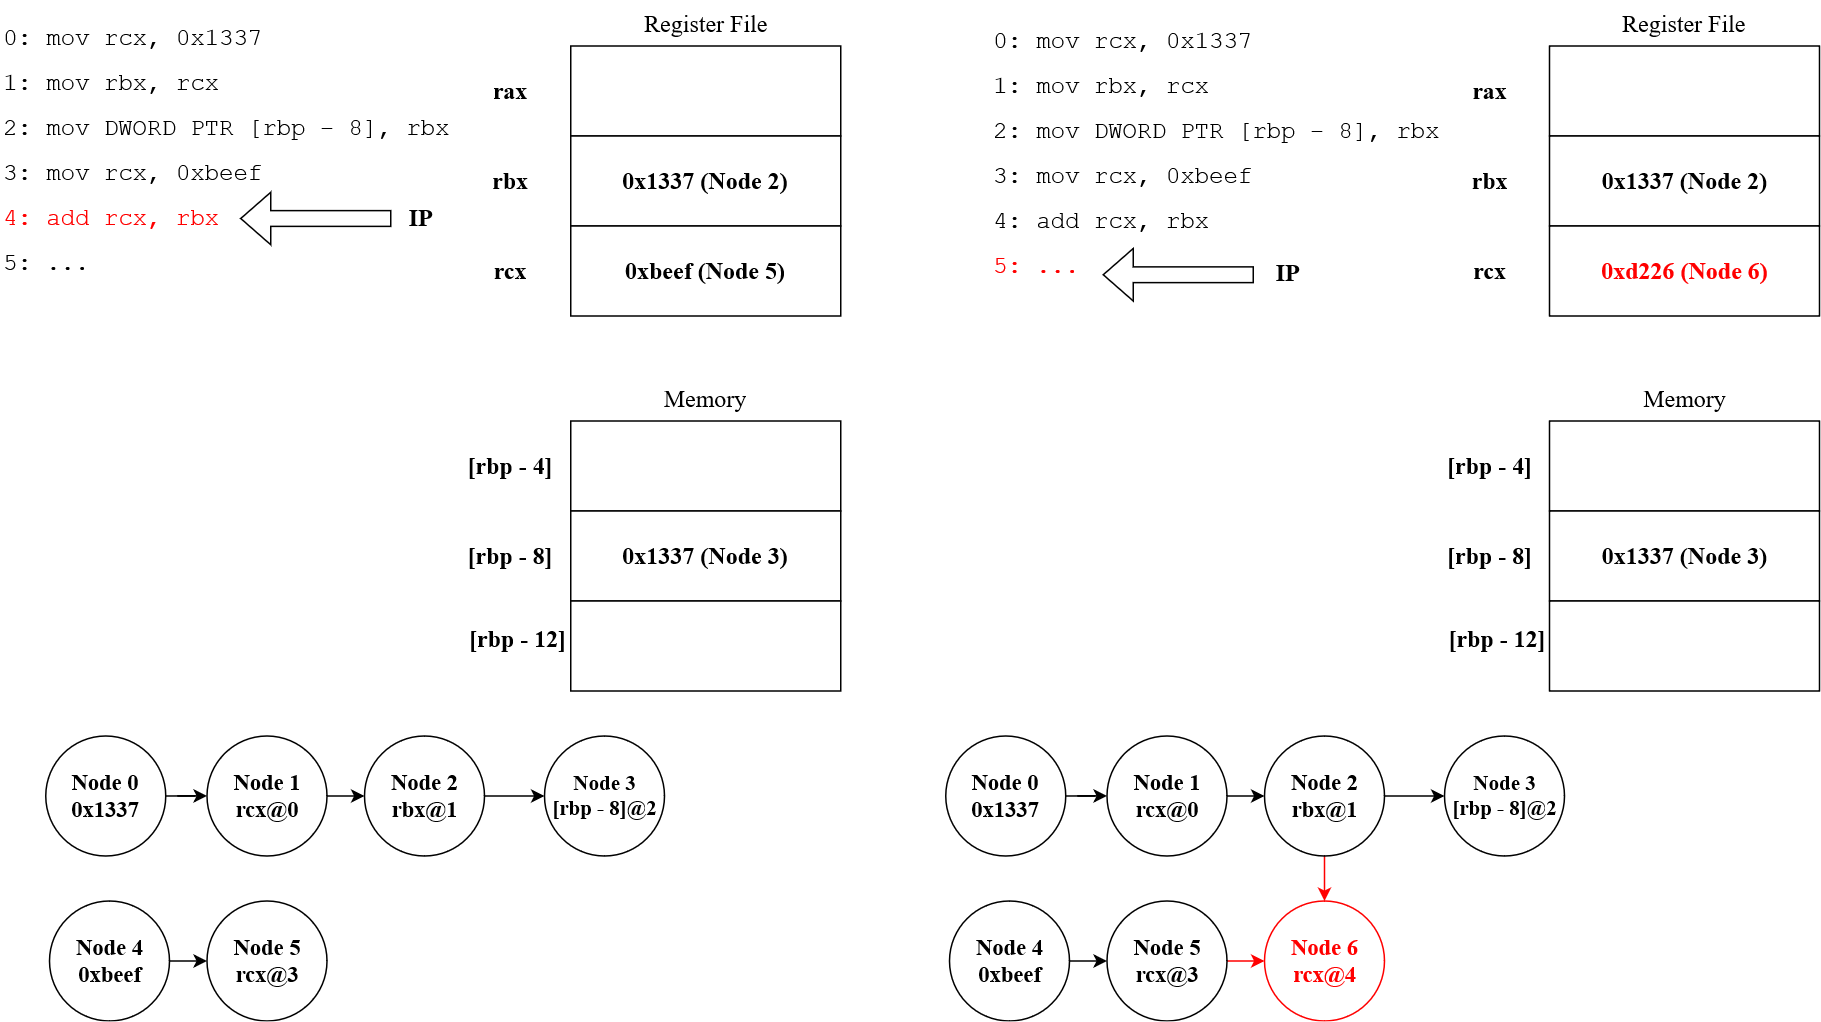
\includegraphics[width=1\maxwidth{\textwidth}]{state.png}
    \caption[Register File and Graph State Before and After Executing Instruction 4]{Register file and graph state before and after executing instruction 4. After executing the addition instruction, a new node for the destination operand is created and linked to the source operands. The register file for the destination operand is also updated to point to this new node.}
    \label{fig:link}
\end{figure}
The program in Figure \ref{fig:link} will be used as a motivating example to explain the linking process. The leftmost diagram gives an overview of the state of the register file, memory, and graph prior to the execution of instruction 4 and will serve as the state that is used to determine dependencies. As an add requires the CPU to read the value from the source operand and target operand, nodes 2 and 5, which are currently associated with \code{rbx} and \code{rcx}, respectively, will be located in the register file and tracked as data sources. Once the addition is calculated by the ALU, the value is then written back to the target operand (\code{rcx}). To facilitate this in the analysis, node 6 is created for \code{rcx} at this state and is linked to its two tracked source nodes as a dependency. As the next operation that utilizes \code{rcx} as an operand should be reliant upon the value of \code{rcx} post-addition, the register file for \code{rcx} is updated to point to node 6.

\section{Visualizing Nodes}
\begin{figure}
    \centering
    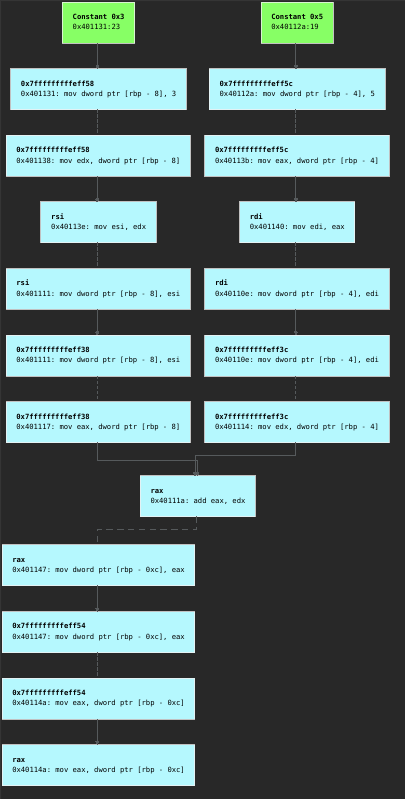
\includegraphics[width=0.6\maxwidth{\textwidth}]{viz.png}
    \caption[{Visualization of a Simple Data Dependency Graph}]{Visualization of a simple data dependency graph. This screenshot is of a subgraph that traces two subsequent additions.}
    \label{fig:viz}
\end{figure}

In addition to implementing the backend analysis for generating a data-dependency graph, its visualization was also within the scope of this thesis. This was accomplished through contribution to \code{angr management}, the official frontend for \code{angr}. An example visualization of a simple data dependency graph is depicted in Figure \ref{fig:viz}.

To improve the user experience, various features were implemented to aid the user in more quickly resolving the dependency of instructions with which they are concerned. For example, search functionality is available to jump through all nodes that match a provided name, instruction address, and/or value. Any of these fields can be omitted in the search, and thus will not be considered in node filtering. In addition to this feature, temporary nodes can be toggled on and off to prevent the screen from being cluttered with useless information when the temporary variables are not relevant to the analysis More importantly, however, the most relevant control is the generation of subgraphs. 

\subsection{Subgraphs}
 A subgraph can be generated from any given node in the data dependency graph. That is, the user can specify to trace the dependency of node X “forwards” and view all nodes that are ancestors of X or trace “backwards” and view all descendants of X. This feature is especially helpful in decreasing screen clutter, as the majority of nodes on a graph will not be relevant to a given dependency trace. 